\documentclass[10pt,letterpaper,onecolumn,draftclsnofoot,journal]{IEEEtran}
\usepackage[margin=0.75in]{geometry}
\usepackage{listings}
\usepackage{color}
\usepackage{longtable}
\usepackage{graphicx}
\usepackage{caption}
\usepackage{float}
\usepackage{tabu}
\usepackage{enumitem}
\usepackage{courier}
\usepackage[hidelinks]{hyperref}

\setlength{\parindent}{0cm}
\setcounter{secnumdepth}{1}

\newcommand{\namesigdate}[2][6cm]{%
	\begin{tabular}{@{}p{#1}@{}}
		#2 \\[3\normalbaselineskip] \hrule \\[0pt]
		{\small \textit{Signature}} 
		\\[2\normalbaselineskip] \hrule \\[0pt]
		{\small \textit{Date}}
	\end{tabular}
}

\begin{document}
\begin{titlepage}
	\title{The ARLISS Project\\Progress Report\\Senior Capstone}
	\author{Steven Silvers\\
		Capstone Group 27\\Winter Term}
	\date{\today}
	\maketitle
	\vspace{4cm}
	\begin{abstract}
		\noindent This document details Steven's experience working on the ARLISS Project during the winter term of 2017. This includes progress made, problems encountered and plans to address those problems as well as plans for future development of the project.
	\end{abstract}

\end{titlepage}
\tableofcontents
\clearpage

\section{Introduction}
\par
This document covers the progress made by our team on the ARLISS Project over the course of winter term. The goal of this project is to work with a team of mechanical engineers and a team of electrical engineers to design and build a miniature rover that will be Oregon State University's entry into the annual ARLISS competition held in September. As part of the competition, the rover must be able to be deployed from a rocket at 10,000 feet AGL, land safely on the ground, unpack from any holding canister, lock on and autonomously drive to a finish destination at a set of provided GPS coordinates. Along the way the rover may encounter various obstacles that it will need to identify and avoid such as rocks or tire ruts.




\section{Summary of Winter Term}


\subsection{Steven Silvers}
This section details the progress made by team member Steven Silvers during the first half of winter term  as well as any work done over winter break. Steven is responsible for making sure the control board for our project will provide what we need, and for determining what kind of wheel system our rover will use. The biggest piece that Steven is responsible for is the obstacle avoidance module, which is the main tool used by our autonomous driving system to keep our rover from becoming stuck during the competition.

\subsection{Week 1}
Start of winter term, over break I studied various autonomous driving methods since that is the main part of the project I am responsible for. I also looked at different hardware implementations and how they would possibly effect our programming decisions. We are communicating with the rest of the ARLISS capstone team to find a weekly meeting time, and have set our weekly TA meeting for Tuesdays at 1:30pm. Hopefully our whole team meeting time will be set soon so the ECE and ME teams can update us on their progress.

\subsection{Week 2}
Week two we met with our TA Franks for the first time this term, and discussed what is expected of the group as far as implementation of our project for this term. We as a group decided what a successful alpha version of our project would look like. We decided since the other two teams on our project would mostly likely not be finished with the hardware implementation until the end of the term, that for our alpha release we would write simulators for our individual modules to demonstrate that they function properly. The goal for the Beta release is to have the code implemented on hardware, but that is entirely dependent on the progress made by the ME and ECE groups.


\subsection{Week 3}
Week three we held a team wide meeting with the ECE and ME groups to better figure out time lines and what everyone is working on. It sounds like the ECE team has finally settled on using a Raspberry Pi zero as the main board for the rover, giving us a better idea of how we need to implement our code. The ME team told us that they will be designing and creating the wheel system in house so that it is fully customized to meet our needs. Progress has continued to be made on developing and simulating our individual code pieces in preparation for the week 6 alpha release.

\subsection{Week 4}
This week was mostly business as usual, we continued working on the alpha version of our project, as well as had an all group meeting that included our client Dr. Squires. My development module has been changed in that it will be getting a .mat file as input instead of a 2d binary array. This change will need to be reflected in the requirements document. As it is a late change, the alpha version will still be making use of a 2D binary array, and the plan is to change over to the .mat file for the beta version.

\subsection{Week 5}
Week five was spent doing work on the alpha version of the modules I am responsible for, mostly the obstacle avoidance system. Because of this modules' complexity it was decided that the alpha would be a lower level "prof of concept" and full functionality would be added by the 1.0 release. I edited both the tech review and the design document to reflect changes that had been made to the project for the sections I am responsible for. The biggest edit was for the control board, reflecting the decision made by the ECE team to use a Raspberry Pi Zero instead of one of the previously listed options.

\subsection{Week 6}
Week six was focused entirely on the upcoming alpha release and progress report. We decided that each team member would write their pieces individually and then combine them into one document Thursday, giving us plenty of time to submit the report on Friday. We got together with the ECE and ME teams for our weekly meeting, which ended early because all three groups were busy with progress reports and had nothing of significance to share. The ME team is uncertain of their capstone number, which hopefully they will figure out soon so that we can register as a group for Expo. The ME team also revealed to us during the short meeting that the rover frame did not hold up in testing and broke. They are now considering manufacturing the frame to the rover out of acrylic as it is a sturdy lightweight material that they believe will be easier to work with.

\section{Modules I Am Responsible For}

\subsection{Control Board}
Progress for the control board module so far consists of coming together with the ECE and ME teams and selecting what board we would like to use for the project. At our first all group meeting we decided that a Raspberry Pi Zero would be the best fit for our project given the size constraints and the processing power needed by our imaging system. Once that decision was made, it was a matter of placing the order for the Pi Zero boards and updating the technology review and the design document to reflect the decision to use the Pi Zero.
\par
The Pi boards arrived shortly after the alpha version was turned in, the ECE team took two to work on building the electronics systems for the rovers while the CS team took one for testing our modules with. Paul held on to the board as he took up the task of doing most of the initial testing on it as well as installing Opencv and the Pi camera. At this point we are waiting on the ECE team to finish installing various sensors on the boards so that we can do testing with live data instead of just random testing with simulated values. We ran into a couple problems with the boards, namely we broke a camera port on one while trying to install the Pi camera. This problem was fixed by ordering a replacement board which arrived within the week. Another problem is that during weeks 9 and 10 the ECE group stopped communicating with either the CS or ME groups about progress and also stopped attending scheduled meetings and build days. This kept us in the dark about the progress of the hardware install on the ECE Pi boards for multiple weeks, and we eventually ended up getting in contact with our client Dr. Squires about the problem, who was able to reach one group member.
\begin{figure}[H]
	\centering
	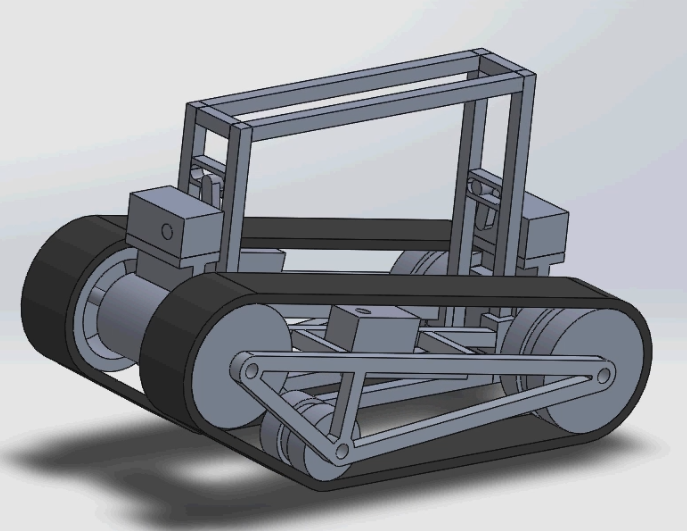
\includegraphics[scale = .4]{Capture.PNG}
	\caption{SolidWorks design of the rover}
	\label{fig:design}
\end{figure}
\subsection{Wheel System}
The wheel system for our rover will be designed and manufactured by our project's ME team here at Oregon State. As shown in figure \ref{fig:design}, our wheel system is a caterpillar track featuring three wheels per track, one of which is connected to a motor while the other two are for stabilization and guidance. Figure \ref{fig:rover} is the finished implementation of the wheel system for our rover, this photo was taken during our week 10 all team meeting. The wheel system was the last piece to get finished for the mechanical team apart from installing electronics, as they had to re-cut the caterpillar track to get a better fit. At this point it is safe to say that the wheel system module is complete and requires no further changes or development.

\begin{figure}[H]
	\centering
	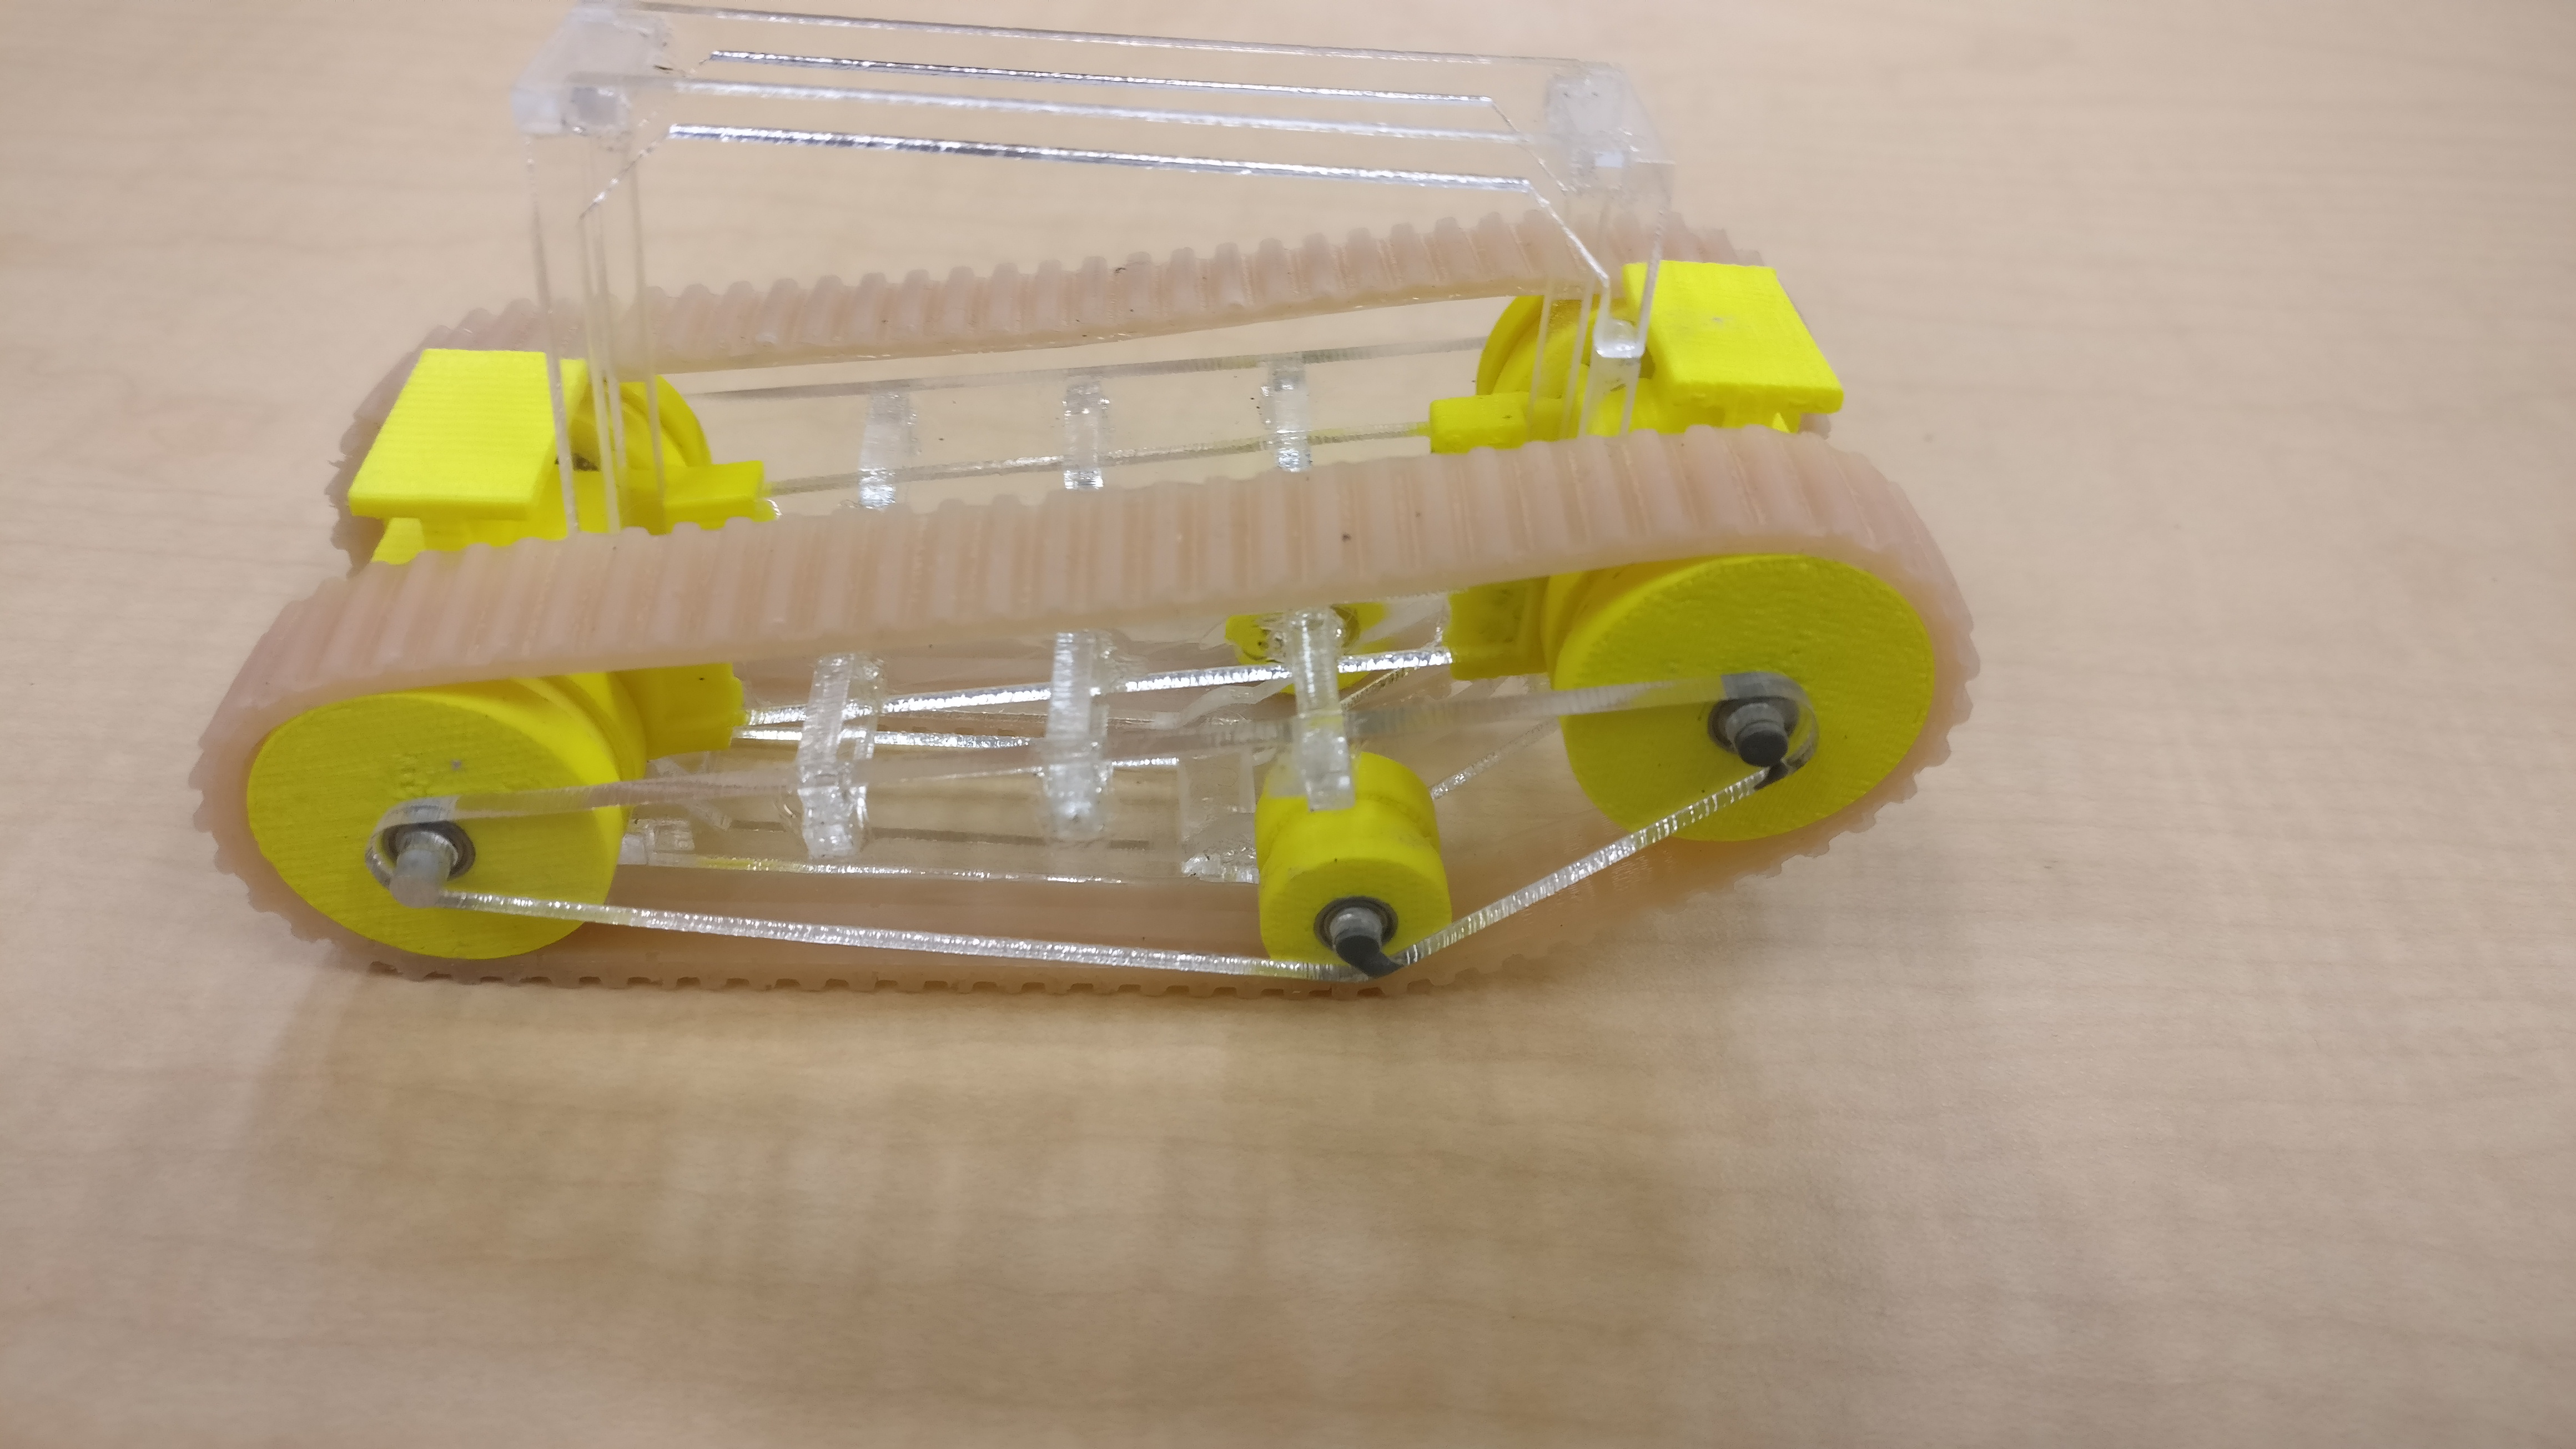
\includegraphics[scale = .05]{builtrover.jpg}
	\caption{Final wheel system}
	\label{fig:rover}
\end{figure}
\subsection{Obstacle Avoidance}
The obstacle avoidance system is what took up most of my time so far this term, as it is proving to be one of the trickier modules. I spent part of winter break as well as the first few weeks of winter term just focused on research for how to best implement a solution to this problem. The initial plan was to take in a 2D binary array as input from the imaging module developed by Zach where ones represent edges detected in an image, and zeros are unchanging terrain.
\begin{figure}[H]
	\centering
	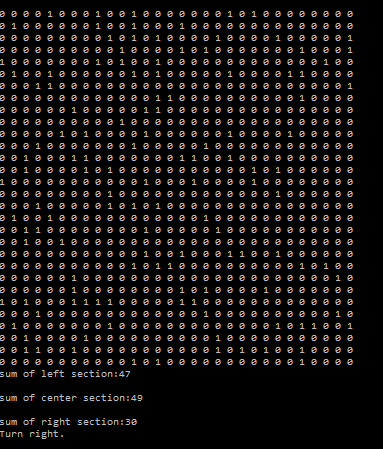
\includegraphics[scale = .75]{obstacleavoidance.png}
	\caption{output from alpha version}
	\label{fig:obstacle}
\end{figure}
\par
The original obstacle avoidance algorithm would splits the array into three large columns, left, center and right, and then sums those columns. This summation tells us where the most edges are, which translates to where the roughest terrain is. In figure \ref{fig:obstacle} it shows that the sum of the right column was the lowest, so the rover should turn right to avoid the rougher terrain in front of it and to the left. For testing purposes, the array used in the alpha release is randomly populated with ones and zeros. The current plan is for the beta version to be tested with actual images to ensure accuracy and logical correctness of the algorithm.

\section{A Reflection of Development Period}
\begin{tabular}{ |p{0.3\linewidth}|p{0.3\linewidth}|p{0.3\linewidth}|  }
	\hline
	\multicolumn{3}{|c|}{Retrospective} \\
	\hline
	Positives& Deltas &Actions \\
	\hline
	Our group works well together. &
	Better understand version control.&
	Each group member will research Github and version control in general. \\
	
	All software components seem possible to implement. &
	Better implement version control &
	Start submitting changes to Github via Pull Request instead of Pushes. \\
	
	The Mechanical Engineering team is very organized and handles the details for the competition. &
	Keep track of project progress better. & Use a separate application to keep track of progress, such as waffle.io.  \\
	\hline
\end{tabular}

\section{Summary of Winter Term Progress}

\section{Team Review}

\section{Conclusion}

\clearpage

\pagenumbering{gobble}
\vspace{1in}

\end{document}
